\chapter{Introduction}\label{chap:intro}
\pagenumbering{arabic}
\setcounter{page}{1}
This document defines the specification of {\XACC} which is an extension of {\XMP} version 1.3\cite{xmp} and {\OACC} version 2.5\cite{openacc}.
{\XACC} provides a parallel programming model for accelerated clusters
which are distributed memory systems equipped with accelerators.
In this document,
terminologies of {\XMP} and {\OACC} are indicated by {\bf bold font}.
For details, refer to each specification\cite{xmp,openacc}.

\section{Hardware Model}
The target of {\XACC} is an accelerated cluster,
a hardware model of which is shown in Fig. \ref{fig:hardware}.

\begin{myfigure}
  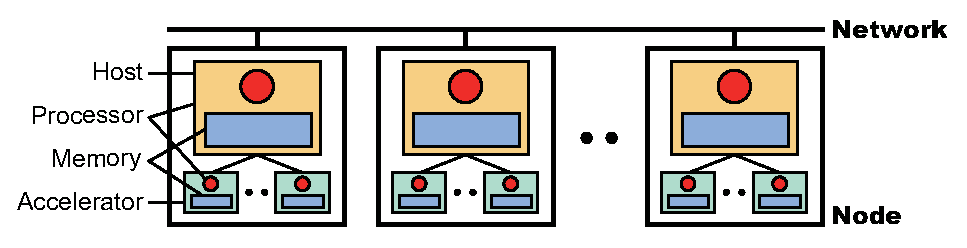
\includegraphics[scale=0.9,clip]{figs/hardware.eps}
  \caption{Hardware Model}\label{fig:hardware}
\end{myfigure}

An execution unit is called {\bf node} as with {\XMP}.
Each {\bf node} consists of a single host and multiple accelerators (such as GPUs and Intel MICs).
Each host has a processor, which may have several cores, and own local memory.
Each accelerator also has them.
Each {\bf node} is connected with each other via network.
Each {\bf node} can access its local memories directly and remote memories,
that is, the memories of another {\bf node} indirectly.
In a host,
the accelerator memory may be physically and/or virtually separate from the host memory as with the memory model of {\OACC}.
Thus,
a host may not be able to read or write the accelerator memory directly.

\section{Programming Model}
{\XACC} is a directive-based language extension based on Fortran 90 and ISO C90 (ANSI C90).
To develop applications on accelerated clusters with ease,
{\XACC} extends {\XACC} and {\OACC} independently as follow:
(1) {\XMP} extensions are to facilitate cooperation between {\XMP} and {\OACC} directives.
(2) {\OACC} extensions are to deal with multiple accelerators.

\subsection{{\XMP} Extensions}
In a program using the {\XMP} extensions,
{\XMP}, {\OACC}, and {\XACC} directives are used.
Fig. \ref{fig:concept} shows a concept of the {\XMP} extensions.

\begin{myfigure}
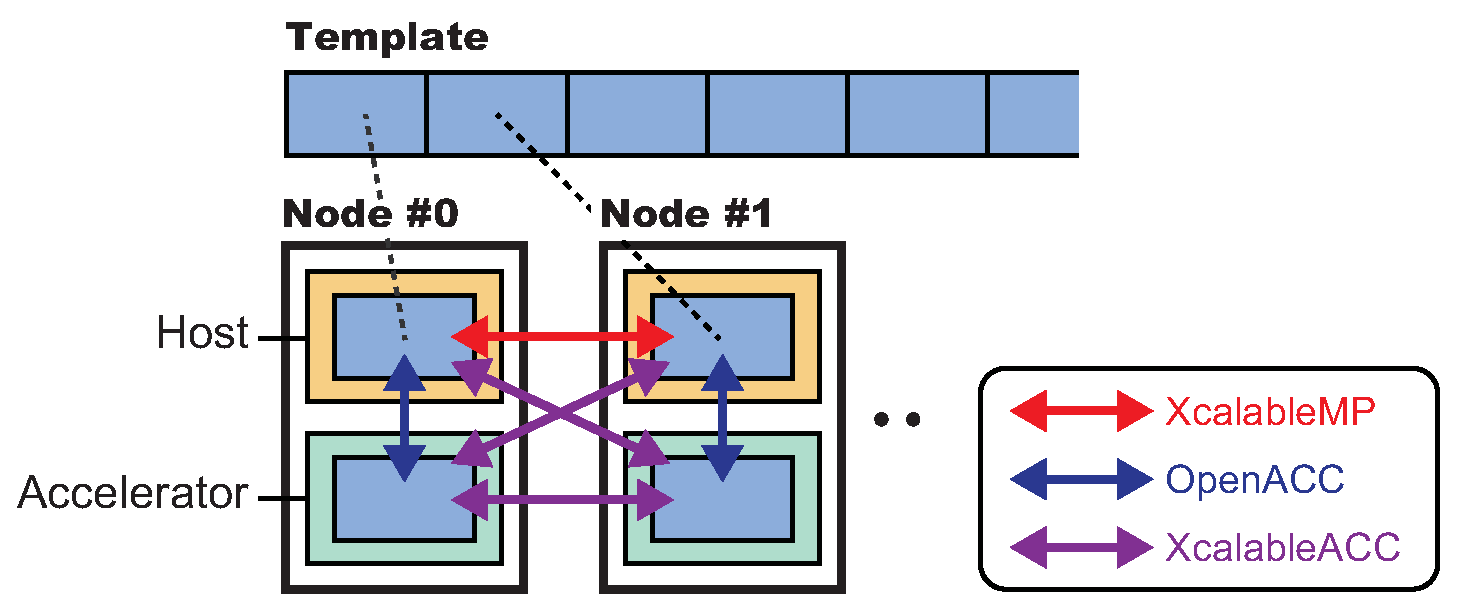
\includegraphics[scale=0.5,clip]{figs/concept.eps}
  \caption{Concept of {\XMP} Extensions}\label{fig:concept}
\end{myfigure}

{\XMP} directives define a {\bf template} and a {\bf node set}.
The {\bf template} represents a global index space, which is distributed onto the {\bf node set}.
Moreover, {\XMP} directives declare {\bf distributed arrays},
parallelize loop statements and transfer data among host memories according to the distributed {\bf template}.
{\OACC} directives transfer the {\bf distributed arrays} between host memory and accelerator memory on the same {\bf node}
and execute the loop statements parallelized by {\XMP} on accelerators in parallel.
{\XACC} directives, which are {\XMP} communication directives with an {\tt acc} clause, 
transfer data among accelerator memories and between accelerator memory and host memory on different {\bf nodes}.
Moreover, 
{\bf coarray} features also transfer data on different nodes.

%The {\XMP} extension is defined to develop parallel applications with keeping the sequential code image.
Note that 
the {\XMP} extensions are not a simple combination of {\XMP} and {\OACC}.
For example, 
if you represent communication of {\bf distributed array} among accelerators shown in Fig. \ref{fig:concept} by the combination of {\XMP} and {\OACC},
you need to specify explicitly communication between host and accelerator by {\OACC} and that between hosts by {\XMP}.
Moreover,
you need to calculate manually indices of the {\bf distributed array} owned by each {\bf node}.
By contrast,
{\XACC} directives can represent such communication among accelerators directly using global indices.

\subsection{{\OACC} Extensions}
The {\OACC} extension can represent offloading works and data to multiple-accelerators on a {\bf node}.
Fig. \ref{fig:concept_acc_ex} shows a concept of the {\OACC} extension.

\begin{myfigure}
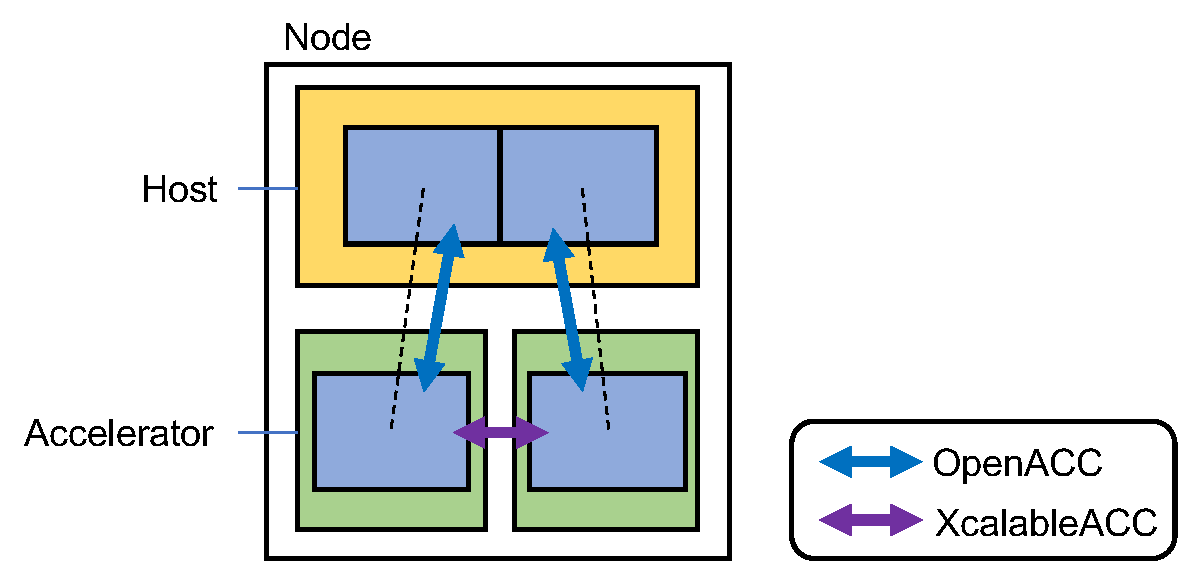
\includegraphics[scale=0.5,clip]{figs/concept_acc_ext.pdf}
  \caption{Concept of {\OACC} Extension}\label{fig:concept_acc_ex}
\end{myfigure}

{\OACC} extension directive defines a {\bf device set}.
The {\bf device set} represents a set of devices on a {\bf node}.
Futher, {\OACC} extension directives declare {\bf distributed arrays} on the {\bf device set} while maintaining the arrays on the host memory, and the directives distribute offloading loop statement and memory copy between host and device memories for the {\bf distributed-arrays}.
Moreover, {\OACC} extension directives synchronizes devices among the {\bf device set}.
{\XACC} directives also transfer data between device memories on the {\bf node}.

\section{Execution Model}
The execution model of {\XACC} is a combination of those of {\XMP} and {\OACC}.
While the execution model of a host CPU programming is based on that of {\XMP},
that of an accelerator programming is based on that of {\OACC}.
Unless otherwise specified,
each {\bf node} behaves exactly as specified in the {\XMP} specification\cite{xmp} or the {\OACC} specification\cite{openacc}.
%For details, refer to each specification\cite{xmp,openacc}.

An {\XACC} program execution is based on the SPMD model, 
where each {\bf node} starts execution from the same main routine and keeps executing the same code independently (i.e. asynchronously), 
which is referred to as the replicated execution
until it encounters an {\XMP} construct or an {\XMP}-extension construct.
In particular,
the {\XMP}-extension construct may allocate, deallocate, or transfer data on accelerators.
An {\OACC} construct or an {\OACC}-extension construct may define {\bf parallel regions}, such as work-sharing loops, 
and offloads it to accelerators under control of the host.

When a {\bf node} encounters a loop construct 
targeted by a combination of {\XMP} {\tt loop} and {\OACC} {\tt loop} directives,
it executes the loop construct in parallel with other {\bf accelerators},
so that each iteration of the loop construct is independently executed by the {\bf accelerator}
where a specified data element resides.

When a {\bf node} encounters a {\XACC} synchronization or a {\XACC} communication directive,
synchronization or communication occurs between it and other accelerators.
That is, such {\bf global constructs} are performed collectively by the {\bf current executing nodes}.
Note that neither synchronizations nor communications occur without these constructs specified.

\section{Data Model}
There are two classes of data in {\XACC}: {\bf global data} and {\bf local data} as with {\XMP}. 
Data declared in an {\XACC} program are local by default.
Both {\bf global data} and {\bf local data} can exist on host memory and accelerator memory.
About the data models of host memory and accelerator memory, refer to the OpenACC specification\cite{openacc}.

{\bf Global data} are ones that are distributed onto the {\bf executing node set} by the {\tt align} directive.
Each fragment of a {\bf global data} is allocated in host memory of a {\bf node} in the {\bf executing node set}.
{\OACC} directives can transfer the fragment from host memory to accelerator memory.

{\bf Local data} are all of the ones that are not global.
They are replicated in the local memory of each of the {\bf executing nodes}.

A {\bf node} can access directly only {\bf local data} and sections of {\bf global data} that are allocated in its local memory.
To access data in remote memory, 
explicit communication must be specified in such ways as the global communication constructs and the {\bf coarray} assignments.

Particularly in {\XACCF}, 
for common blocks that include any global variables, 
the ways how the storage sequence of them is defined and how the storage association of them is resolved are implementation-dependent.

\section{Directive Format}
This section describes the syntax and behavior of {\XMP} and {\OACC} directives in {\XACC}.
In this document, 
the following notation is used to describe the directives.

\vspace{0.5cm}%
\begin{tabular}{ll}
{\tt xxx} & {\tt type-face} characters are used to indicate literal type characters. \\
{\it xxx...} & If the line is followed by ``...'', then xxx can be repeated. \\
{\it [xxx]} & {\it xxx} is optional. \\
{\bsquare} & The syntax rule continues. \\
\verb![F]! & The following lines are effective only in {\XACCF}. \\
\verb![C]! & The following lines are effective only in {\XACCC}. \\
\end{tabular}
\vspace{0.5cm}%

In {\XACCF}, 
{\XMP} and {\OACC} directives are specified using special comments that are identified by unique sentinels {\tt\verb|!$xmp|} and {\tt\verb|!$acc|} respectively.
the directives follow the rules for comment lines of either the Fortran free or fixed source form,
depending on the source form of the surrounding program unit\footnote{Consequently, the rules of comment lines that an
{\XMP} directive follows is the same as the ones that an {\OMP} directive follows.}.
The directives are case-insensitive.

\vspace{0.5cm}
\Syntax{directive}
\begin{tabular}{ll}
\verb![F]! & \verb|!$xmp| {\it directive-name clause} \\
\verb![F]! & \verb|!$acc| {\it directive-name clause} \\
\end{tabular}
\vspace{0.5cm}

In {\XACC}, 
{\XMP} and {\OACC} directives are specified using the \verb|#pragma| mechanism provided by the C standards.
the directives are case-sensitive.

\vspace{0.5cm}
\Syntax{directive}
\begin{tabular}{ll}
\verb![C]! & \verb|#pragma xmp| {\it directive-name clause} \\
\verb![C]! & \verb|#pragma acc| {\it directive-name clause} \\
\end{tabular}
\vspace{0.5cm}

%Directives are classified as {\bf declarative directives} and {\bf executable directives}\cite{xmp}.
%
%The {\bf declarative directives} are {\tt nodes}, {\tt template}, {\tt distribute}, {\tt align},
%{\tt shadow}, {\tt coarray}, {\tt declare}, and {\tt routine} directives.
%
%The {\bf executable directives} are {\tt template\_fix}, {\tt task}, {\tt tasks}, {\XMP} {\tt loop}, 
%{\tt array}, {\tt reflect}, {\tt reflect\_init}, {\tt reflect\_do}, {\tt gmove}, {\tt barrier}, 
%{\tt reduction}, {\tt bcast}, {\tt wait\_async},
%{\tt parallel}, {\tt kernels}, {\tt data}, {\tt host\_data}, {\OACC} {\tt loop},
%{\tt cache}, {\tt atomic}, {\tt init}, {\tt shutdown}, {\tt set}, {\tt update}, 
%{\tt wait}, {\tt enter\_data}, and {\tt exit\_data} directives.
%An {\bf executable directive} and its associated user code make up an {\XACC} construct, 
%as in the following format:
%
%\vspace{0.5cm}
%\begin{tabular}{ll}
%\verb![F]! & \verb|!$xmp| {\it directive-name clause} ...\\
% & \hspace{0.5cm} {\it structured-block} \\
%\verb![F]! & \verb|!$acc| {\it directive-name clause} ...\\
% & \hspace{0.5cm} {\it structured-block} \\
%\end{tabular}
%
%\vspace{0.3cm}
%
%\begin{tabular}{ll}
%\verb![C]! & \verb|#pragma xmp| {\it directive-name clause} ...\\
% & \hspace{0.5cm} {\it structured-block} \\
%\verb![C]! & \verb|#pragma acc| {\it directive-name clause} ...\\
% & \hspace{0.5cm} {\it structured-block} \\
%\end{tabular}
%\vspace{0.5cm}

\section{Organization of This Document}
The remainder of this document is structured as follows:

\begin{itemize}
 \item Chapter 2: {\XMP} Extensions
 \item Chapter 3: {\OACC} Extensions
\end{itemize}
